\documentclass[12pt]{article}
\usepackage[utf8]{inputenc}
\usepackage{caption}
\usepackage{times}
\usepackage{graphics}
\usepackage{graphicx}
\usepackage{float}
\usepackage{hyperref}
\usepackage{listings}
\hypersetup{
	colorlinks=true,
	linkcolor=blue,
	filecolor=magenta,      
	urlcolor=cyan,
}

\title{Docker inrichten}
\author{Thomas van Dongen, Koen Schilders}
\date{28 februari 2018}

\begin{document}


% De titelpagina
\begin{titlepage}
\maketitle
\end{titlepage}



% Hier wordt beschreven hoe we Docker opzetten voor CI/CD
% Link naar tutorial: https://blog.philipphauer.de/tutorial-continuous-delivery-with-docker-jenkins/
\section{Opzet CI/CD met Docker}
Voor deze opdracht moeten we een skelet opzetten van een CI/CD pipeline met Docker. De pipeline bestaat uit twee Docker containers. Het ene container test de build en maakt een Docker image, de andere container deployed de container en draait de applicatie. De pipeline is uitgewerkt in Figure \ref{fig:cicd_pipeline}.
\newline
\begin{figure}[H]
	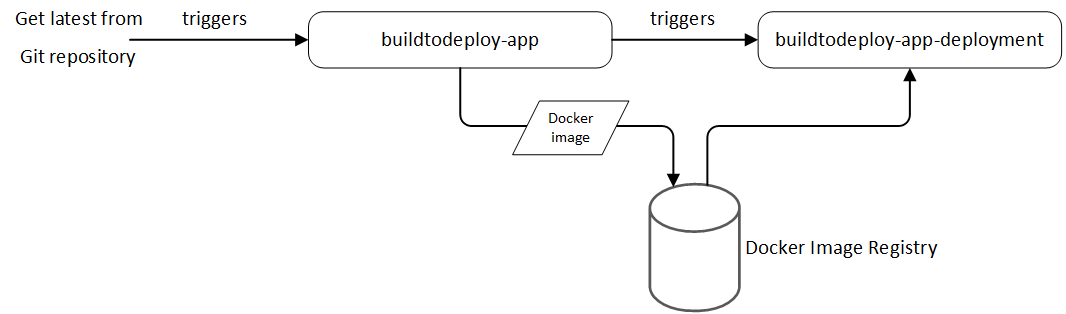
\includegraphics[width=\textwidth]{images/DockerPipeline.png}
	\caption{De pipeline van Docker containers\label{fig:cicd_pipeline}}
\end{figure}

\subsection{Git repository}
Eerst gaan we een Git repository maken met een test applicatie. De applicatie is een simpele rekenmachine met enkele JUnit-tests (Figure \ref{fig:calculator_app}).

\begin{figure}[H]
	\begin{center}
		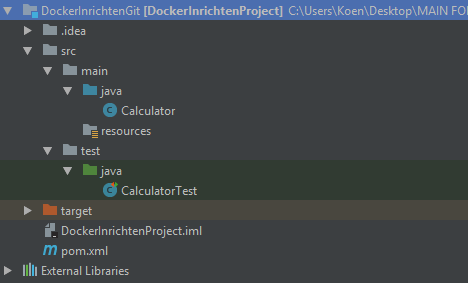
\includegraphics[width=0.75\textwidth]{images/CalculatorApplication.png}
		\caption{De structuur van de Calculator applicatie\label{fig:calculator_app}}
	\end{center}
\end{figure}

De Git repository heeft alleen een master branch. Dit is prima voor nu, maar in een echt project is het beter om het systeem van branches uit het releaseplan te gebruiken. Dat branch systeem is ingericht voor CI/CD gebruik.

\subsection{Jenkins container}
Nu gaan we een Docker container maken waar Jenkins op draait. Deze container moet zo worden ingericht dat Jenkins de Git repository weet te vinden, de tests gedraaid worden, en uiteindelijk een nieuwe Docker container aanroept.
\linebreak
In plaats van op een schone container Jenkins te installeren maken we gebruik van de kracht van Docker. Op de Docker Hub is een kant-en-klare Jenkins image te vinden. Deze kan gepulled worden met het volgende commando:

\begin{lstlisting}[language=Bash]
    $ docker pull jenkins/jenkins
\end{lstlisting}

\noindent We kunnen de image openen met het volgende commando:

\begin{lstlisting}[language=Bash]
    $ docker run -p 8080:8080 -p 50000:50000 jenkins/jenkins
\end{lstlisting}

\noindent De docker instance draait, en heeft poort 8080 opengezet, zoals we hadden meegegeven in het commando. Nu moeten we het IP weten van Docker. Bij Docker Legacy is dit niet localhost, maar een ander local IP. Dit is op te vragen met het commando:

\begin{lstlisting}[language=Bash]
    $ docker-machine ip
\end{lstlisting}

\noindent Door naar het geretourneerde IP + poort 8080 te gaan in de browser kunnen we Jenkins configureren. Hiervoor moet een wachtwoord ingevoerd worden, welke te vinden is in de console window.

% TODO: Jenkins configureren tekst

Na het configureren moeten we de image opslaan. Als we dit niet doen zijn we alle wijzigingen kwijt. Dit kan door het volgende commando uit te voeren, waarbij CONTAINER vervangen dient te worden met het ID van de container:

\begin{lstlisting}[language=Bash]
    $ docker commit CONTAINER jenkins/jenkins:configured
\end{lstlisting}

% TODO: Meer tekst


\begin{figure}[H]
	\begin{center}
		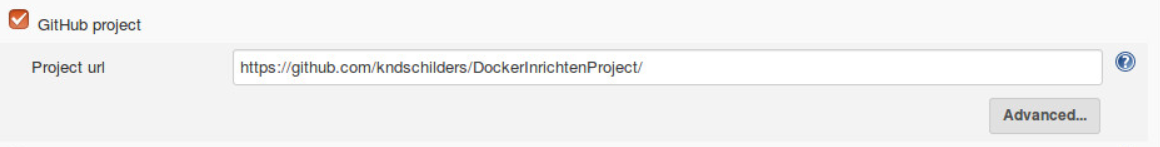
\includegraphics[width=1.0\textwidth]{images/Jenkins-Github.PNG}
		\caption{GitHub repository instellen\label{fig:jenkins_config_repo}}
	\end{center}
\end{figure}

\begin{figure}[H]
	\begin{center}
		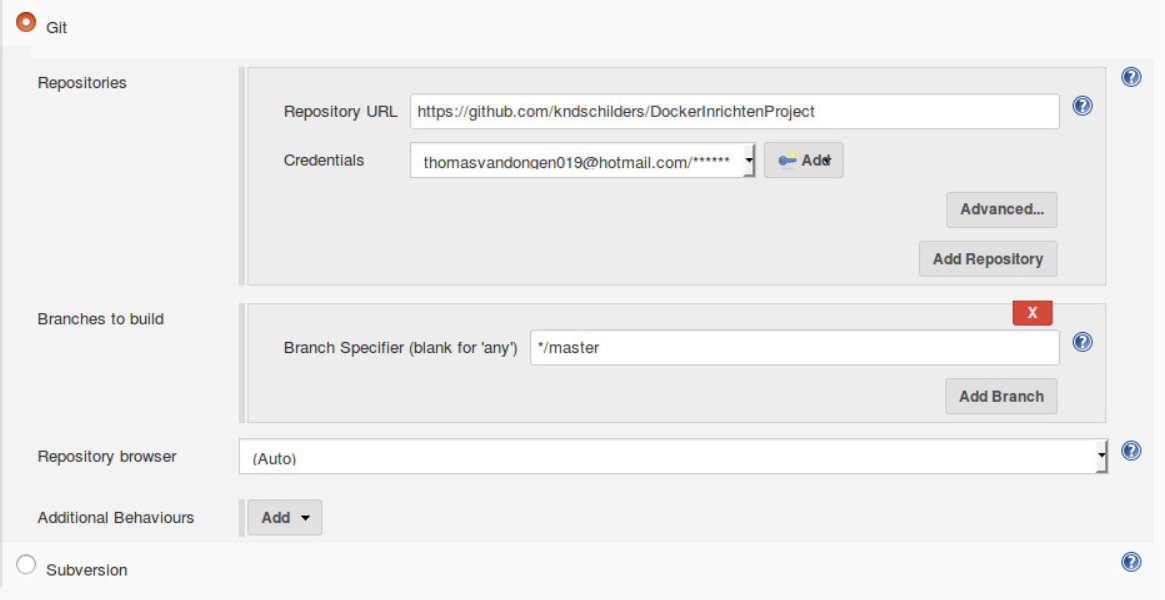
\includegraphics[width=1.0\textwidth]{images/Jenkins-Github-2.PNG}
		\caption{GiHub instellen\label{fig:jenkins_config_repo_2}}
	\end{center}
\end{figure}

\begin{figure}[H]
	\begin{center}
		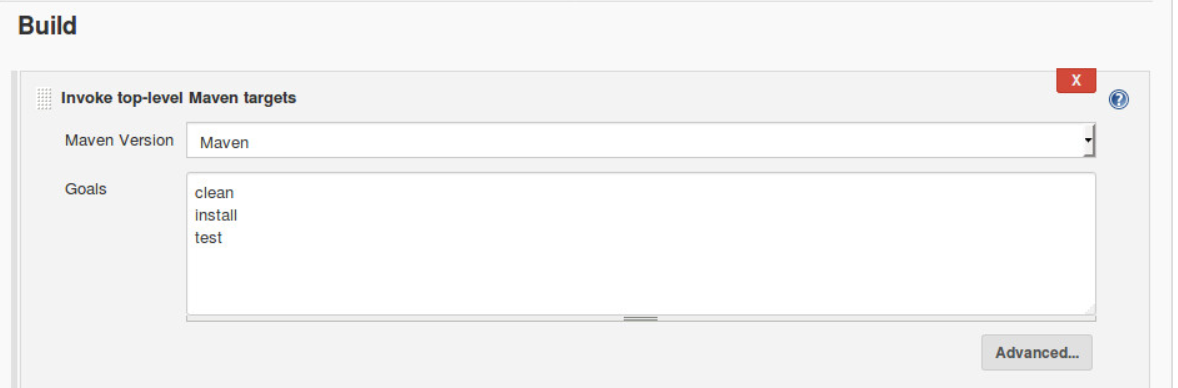
\includegraphics[width=1.0\textwidth]{images/Maven.PNG}
		\caption{Maven instellen\label{fig:jenkins_maven}}
	\end{center}
\end{figure}

\begin{figure}[H]
	\begin{center}
		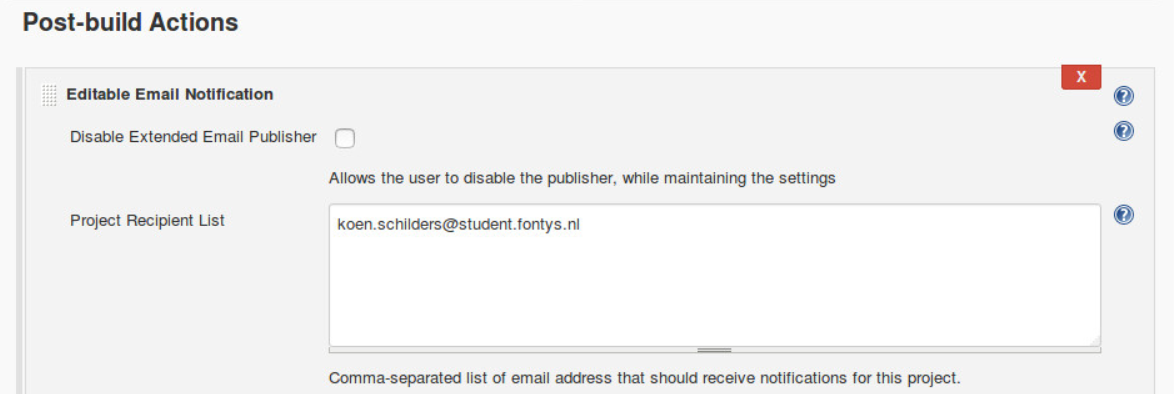
\includegraphics[width=1.0\textwidth]{images/Postbuildaction.PNG}
		\caption{Email notifications instellen\label{fig:jenkins_config_email_notifications}}
	\end{center}
\end{figure}


\subsection{Deployment container}
De Jenkins container is klaar, en de image (een war-file) wordt naar de Docker image repository gestuurd. Nu moet de image nog draaien in een aparte container, de deployment container.

We hebben gekozen om de war-file in een Tomcat container te draaien. 

%TODO:
% TomcatGlassfish docker image pullen en inrichten

% Eventueel: NAT instellingen controleren als dat nodig is

% Deployen

% Applicatie bereiken vanaf andere computer


% Sources
\begin{thebibliography}{9}
	\bibitem{shortcode_name}
		Name of author,
		\textit{Title of page or book},
		Date of publication,
		\url{https://google.com}
\end{thebibliography}
\end{document}